\documentclass[handout]{beamer}
\usetheme[]{Szeged}
\usecolortheme{beaver}
\setbeamertemplate{footline}[frame number]
\usepackage[utf8]{inputenc}
\usepackage[spanish,es-nodecimaldot]{babel}
\usepackage{amsmath, amsthm, amsfonts, amssymb}
\usepackage{textcomp}
\usepackage{multimedia}
\DeclareGraphicsExtensions{.png,.pdf,.jpg,.jpeg}
\graphicspath{{imagenes/}} %directorio donde se guardan las imagenes
\usepackage{hyperref}
\usepackage{enumitem}

\SetLabelAlign{parright}{\parbox[t]{\labelwidth}{\raggedleft#1}}
\setlist[description]{style=multiline,topsep=10pt,leftmargin=4cm,align=parright}
\setlist[itemize]{label=\textbullet}

\title{Física II}
\author{Introducción a Fluidos}
\institute[UVM]{4\textdegree \hspace{2pt} cuatrimestre.}
\logo{
\includegraphics[width=1.2cm]{uvm}}
% \date{\today}

\begin{document}

\begin{frame}[noframenumbering]
  \titlepage
  \begin{center}
    
\includegraphics[width=5.5cm]{uvm1}    
  \end{center}  
\end{frame}




\begin{frame}
  \frametitle{Estados de la materia}
  \begin{itemize}
  \item Sólido.
  \item Líquido.
  \item Gaseoso.
  \end{itemize}

  \begin{block}{Como se ve un átomo}
    \href{https://www.youtube.com/watch?v=yqLlgIaz1L0}{Link}
  \end{block}

  \begin{block}{Estados de la materia}
    \href{https://www.youtube.com/watch?v=s-KvoVzukHo}{Link}
  \end{block}

  
\end{frame}



\begin{frame}
  \frametitle{Sólidos}

  \begin{block}{Propiedades visibles}
    \begin{itemize}
    \item Rígidos
    \item Forma fija
    \item Volumen fijo
    \end{itemize}
  \end{block}

  \begin{block}{Propiedad no visible}
    La energía cinética de las moléculas es menor que la energía potencial (cohesión) que
    existe entre ellas.
  \end{block}
  
\end{frame}

\begin{frame}
  \frametitle{Líquidos}

  \begin{block}{Propiedades visibles}
    \begin{itemize}
    \item No son rígidos.
    \item No tiene una forma fija.
    \item Tienen volumen fijo.
    \end{itemize}
  \end{block}

  \begin{block}{Propiedad no visible}
    La energía cinética de las moléculas es aproximademente igual que la energía potencial
    (cohesión) de sus moléculas.
  \end{block}
  
\end{frame}



\begin{frame}
  \frametitle{Gases}

  \begin{block}{Propiedades visibles}
    \begin{itemize}
    \item No son rígidos.
    \item No tiene una forma fija.
    \item No tiene un volumen fijo.
    \end{itemize}
  \end{block}

  \begin{block}{Propiedad no visible}
    La energía cinética de las moléculas es mayor que la energía potencial
    (cohesión).
  \end{block}
  
\end{frame}



\section{Hidráulica}

\begin{frame}
  \frametitle{Hidráulica}  
  \begin{block}{La hidráulica}
    es la parte de la física que estudia la mecánica de los líquidos.
  \end{block}
  \begin{description}
  \item[Hidrostática:] Estudia los líquidos en reposo.
  \item[Hidrodinámica:] Estudia el comportamiento de los líquidos en movimiento
  \end{description}

  \begin{block}{Se considera que los líquidos son}
    \begin{description}
    \item[Isótropos] Las mismas propiedades físicas en todas direcciones.
    \item[Incomprensibles] El volumen no cambia.
    \item[Totalmente fluidos] Sus moléculas atraviesan una sección a la misma velocidad y
      de manera continua.
    \end{description}
  \end{block}
\end{frame}

\section{Hidrostática}

\begin{frame}
  \frametitle{Propiedades de los fluidos}
  \begin{description}
  \item[Viscosidad] Resistencia que opone un líquido a fluir.
  \item[Tensión superficial] La superficie libre de un líquido se comporte como membrana.
  \item[Cohesión ] Fuerza que mantiene unida a dos moléculas de una misma sustancia
  \item[Adherencia] Fuerza de atracción entre las moléculas de sustancias diferentes.
  \item[Capilaridad] \href{https://www.youtube.com/watch?v=s-KvoVzukHo}{Contacto entre el líquido y una pared solida.}
  \item[Incompresibilidad] Los líquidos tienen volumen fijo.
  \end{description}
\end{frame}

\begin{frame}
  \frametitle{Densidad}

  \begin{block}{Densidad}
    {\huge
      \[\rho = \frac{m}{V}\]}
  \end{block}
  \begin{tabular}{ll}
    $m:$ & Masa (kg)  \\ 
    $V:$ & Volumen (m$^3$) \\ 
    $\rho:$ & Densidad (kg/m$^3$) \\
  \end{tabular}

\end{frame}


\begin{frame}
  \frametitle{Peso específico}

  \begin{block}{Peso específico}
      {\huge
      \[P_{e} = \frac{P}{V}\]}
  \end{block}
  \begin{tabular}{ll}
    $P:$ & Peso (N) \\
    $V:$ & Volumen (m$^3$) \\
    $P_{e}:$ & Peso específico (N/m$^3$) \\
  \end{tabular}    

\end{frame}


\section{Ejercicios}
\begin{frame}
\frametitle{Ejercicios resueltos}
\begin{enumerate}
\item Convertir 50 m$^3$ a cm $^3$
\item De la fórmula de la densidad despejar el volumen.
\item Obtener el peso específico en función de la densidad.
\item Calcular el volumen de un cubo de 2 cm de lado.
\item El volumen de un trozo de oro es de 2.587 cm$^3$, mientras que su masa es 50
  g. Obtener su densidad.
\item ¿Qué volumen debe de tener un tanque para que pueda almacenar 2040 kg de gasolina
  cuya densidad es de 680 kg/m$^3$?
\end{enumerate}
\end{frame}



\section{Presión}
\begin{frame}
  \frametitle{Presión}
  \begin{block}{Presión}
    {\huge
      \[ P = \frac{F}{A}\]}
  \end{block}
  \begin{tabular}{ll}
    $P:$ & Fuerza perpendicular a la superficie(N) \\
    $A:$ & Área sobre la que actua la fuerza (m$^2$) \\
    $F:$ & Presión (N/m$^2$) \\
  \end{tabular}
  \begin{block}{}
    A las unidades N/m$^2$ se les conoce como Pascales (Pa).
  \end{block}
\end{frame}

\begin{frame}
  \frametitle{Diferentes tipos de presiones}
  \begin{description}
  \item[Hidrostática] Originada por el líquido en todos los puntos del líquido y las
    paredes del recipiente que lo contine.
  \item[Atmosférica] Debida a toda la mezcla de gases que hay en la atmósfera.
  \item[Manométrica] Es la presión diferente de la atmósferica.
  \item[Absoluta] Es la suma de la presión manométrica y atmósferica.
  \end{description}
\end{frame}


\begin{frame}
  \frametitle{Presión hidrostática}
  
  \begin{block}{Presión}
    {\huge
      \[ P_{h} = P_{e}h\]}
  \end{block}
  \begin{tabular}{ll}
    $P_{e}:$ & Peso específico (N/m$^3$) \\
    $h:$ & Profundidad o altura del líquido (m) \\
    $P_{h}:$ & Presión hidrostática (Pa) \\
  \end{tabular}
\end{frame}


\begin{frame}
  \frametitle{Paradoja de Stevin}
  {\large ¿En dónde es mayor la presión hidróstatica?}
  \begin{center}
    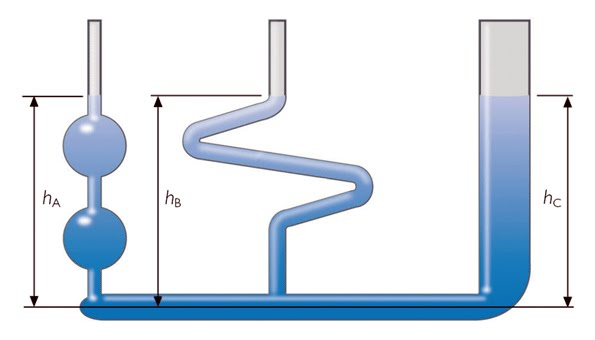
\includegraphics[width=7cm]{vasos_comunicantes}
  \end{center}
\end{frame}


\begin{frame}[allowframebreaks,t]
  \frametitle{Ejercicios resueltos}
  \begin{enumerate}
  \item Si 300 cm$^3$ de alcohol tienen una masa de 237 g, calcular;
    \begin{enumerate}
    \item el valor de su densidad expresada en g/cm$^3$ y kg/m$^3$.
    \item su peso específico expresado en N/m$^3$.  
    \end{enumerate}
  \item Una persona de 60 kg al estar parada sobre el suelo con los pies juntos, ocupa un
    área de 370 cm$^2$. ¿Cuál es la presión ejercida sobre el suelo?
    \begin{enumerate}
    \item en pascales.
    \item en kilopascales.
    \item en kg$_{f}$/cm$^2$
    \end{enumerate}
  \item Sobre un líquido encerrado en un recipiente se aplica una fuerza cuya magnitud es
    de 90 N mediante un pistón de área igual a 0.01m$^2$. ¿Cuál es el valor de la presión?
  \item Calcular la presión hidrostática en el fondo de una alberca de 4 m. La densidad de
    agua es de 1000 kg/m$^3$.
  \end{enumerate}
\end{frame}


\begin{frame}[allowframebreaks,t]
  \frametitle{Ejercicios propuestos}
  \begin{enumerate}
  \item 1500 kg de plomo ocupan un volumen de 0.13274 m$^3$. ¿Cuánto vale su densidad y su
    peso específico?
  \item Una caja metálica ejerce un peso de 300 N sobre el suelo. El área de contacto con
    el suelo es de 3.5 m$^2$. Calcula la presión ejercida por la caja sobre el
    suelo. Expresa el resultado en Pa y kPa.
  \item Determina la presión hidróstatica que ejerce una columna de aceite de 0.4 m, encerrada en un
    tubo, sobre el fondo del tubo. El $P_{e}$ del aceite es 8967 N/m$^3$.
  \item Determina a qué profundidad esta sumergido un buceador en el mar, si soporta un
    presión hidróstatica de 420322 N/m$^2$. ¿Cuál es l presión absoluta que soporta? $\rho_{mar} = 1020 $ kg/m$^3$. 
  \item ¿Cuál es la masa y el peso de 5 litros de mercurio? $\rho_{Hg} = 13600$ kg/m$^3$.
  \item ¿Cuántas barra de hierro puede soportar un camión de 10 toneladas, si cada barra
    tiene un volumen de 0.0106 m$^3$? $\rho_{hierro} = 7860$ kg/m$^3$
  \item ¿Qué es numéricamente mayor la densidad de un objeto o su peso específico?
  \end{enumerate}
\end{frame}

\end{document}